\section{Results}\label{sec:results}

\subsection{How much does the distance metric matter?}

Figure~\ref{fig:vignettes} illustrates the difference between the two local environments for three contrasting
fabrics. In Goi\^ania's planned grid the area reachable within 2~km on foot fills much of the 2-km circle. In the
hillside neighbourhoods of Rio de Janeiro and in Salvador, whose street network is organised around ridges and
valleys, it covers a small, irregular part of it.

\begin{figure}[htbp]
\centering
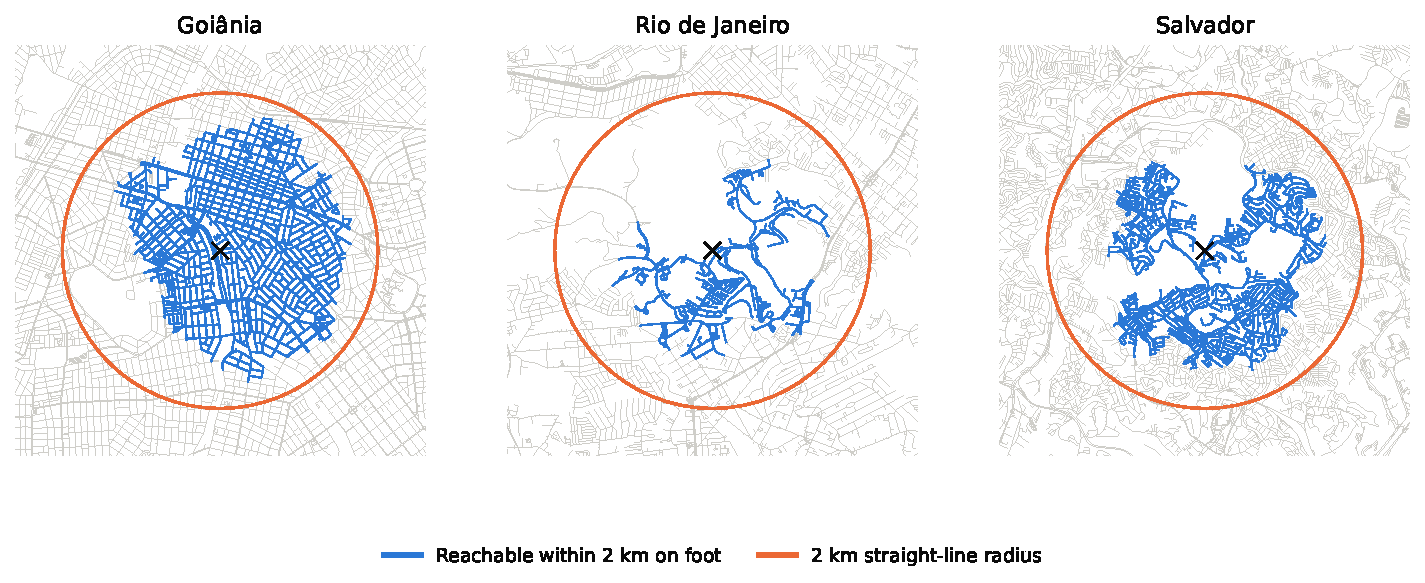
\includegraphics[width=\textwidth]{figures/fig1_vignettes.pdf}
\caption{Street segments reachable within 2~km on foot (blue) and the 2-km straight-line radius (orange) from
the node nearest the population-weighted centre of each city's urban tracts.}\label{fig:vignettes}
\end{figure}

Table~\ref{tab:gap} summarises the comparison for the main specification. Measured with network distance, the
spatial information theory index is higher in all \nCities{} municipalities (\sharePositive\%). The mean index
rises from \meanHeuc{} to \meanHnet{}, a mean relative increase of \meanPdH\%, larger than the $\approx$20\%
reported for US metropolitan areas by \citet{knaap2024segregated}. The relative gap ranges from \minPdH\% to
\maxPdH\%. Levels of racial segregation measured by $H$ are low in absolute terms, as expected for a
five-group index in cities where most residents are \emph{pardo} or white. The two measures are strongly
correlated across cities (Pearson \pearsonMain, Spearman \spearmanMain, Figure~\ref{fig:scatter}).

\begin{table}[htbp]
\centering\small
\caption{Spatial information theory index under Euclidean and network distance (2-km linear kernel,
\nCities{} municipalities). Gap $= H^{N} - H^{E}$; Gap (\%) $= 100\,(H^{N} - H^{E})/H^{E}$.}\label{tab:gap}
\begin{tabular}{lrrrrrrrr}
\toprule
 & count & mean & std & min & 25\% & 50\% & 75\% & max \\
\midrule
H, Euclidean & 91.000 & 0.022 & 0.017 & 0.001 & 0.009 & 0.017 & 0.032 & 0.072 \\
H, network & 91.000 & 0.028 & 0.020 & 0.002 & 0.011 & 0.022 & 0.040 & 0.079 \\
Gap & 91.000 & 0.005 & 0.005 & 0.000 & 0.002 & 0.004 & 0.007 & 0.026 \\
Gap (\%) & 91.000 & 29.835 & 18.968 & 0.751 & 16.294 & 25.209 & 39.522 & 108.987 \\
\bottomrule
\end{tabular}

\end{table}

\begin{figure}[htbp]
\centering
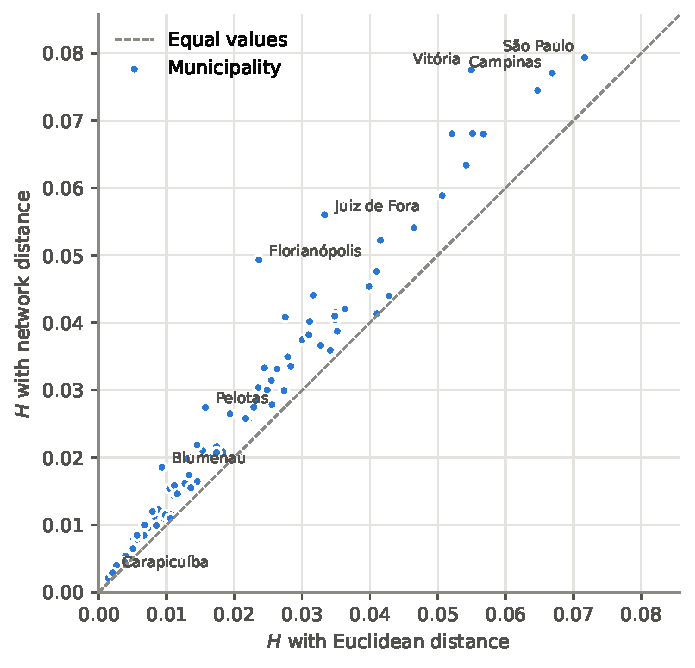
\includegraphics[width=0.6\textwidth]{figures/fig3_scatter.pdf}
\caption{$H$ under Euclidean and network distance. Points above the dashed line are cities where network
distance yields higher segregation. Labelled: the five largest relative gaps and the three highest network
values.}\label{fig:scatter}
\end{figure}

Despite the high correlation, the choice of metric changes the answer to the question most often asked of
segregation indices: which places are most segregated. Among the cities that rank in the top 15 under either
metric, \nRankChangeTop{} change position (Figure~\ref{fig:ranks}). The largest moves are cities built on
hills, islands and narrow valleys: Florian\'opolis rises from 38th to 13th, Juiz de Fora from 22nd to 10th and
Vit\'oria from 6th to 2nd. Bras\'ilia (11th to 17th) and Santos (13th to 20th) fall. The map in
Figure~\ref{fig:map} shows no simple regional pattern in the relative gap. Large gaps occur in the South (Florian\'opolis,
Blumenau, Pelotas), in Minas Gerais (Juiz de Fora), in peripheral municipalities of the S\~ao Paulo and Belo Horizonte
metropolitan areas (Carapicu\'iba, Diadema, Ribeir\~ao das Neves) and in Macei\'o.

\begin{figure}[htbp]
\centering
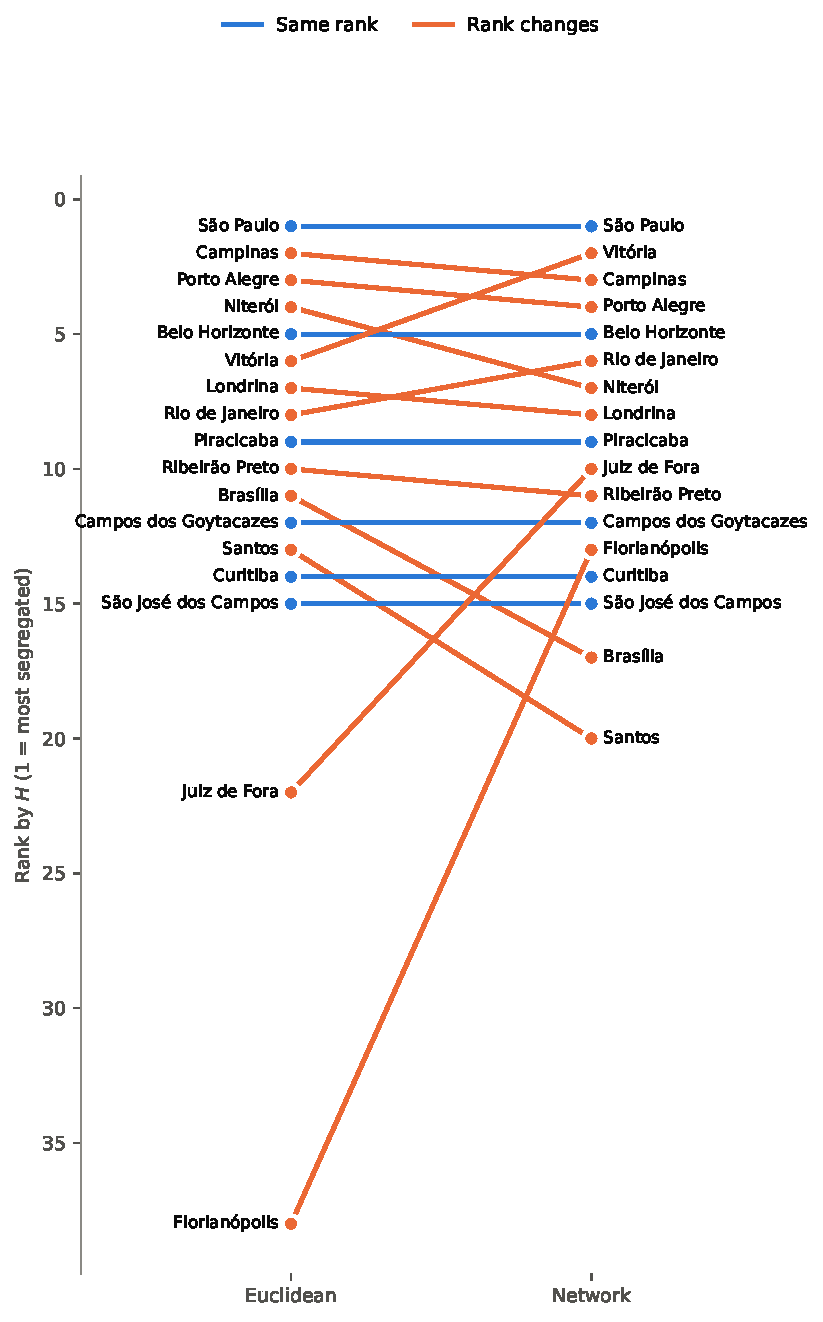
\includegraphics[width=0.62\textwidth]{figures/fig2_rank_slope.pdf}
\caption{Ranks of the most segregated municipalities (top 15 under either metric) with Euclidean and network
distance. Orange lines mark cities whose rank changes.}\label{fig:ranks}
\end{figure}

\begin{figure}[htbp]
\centering
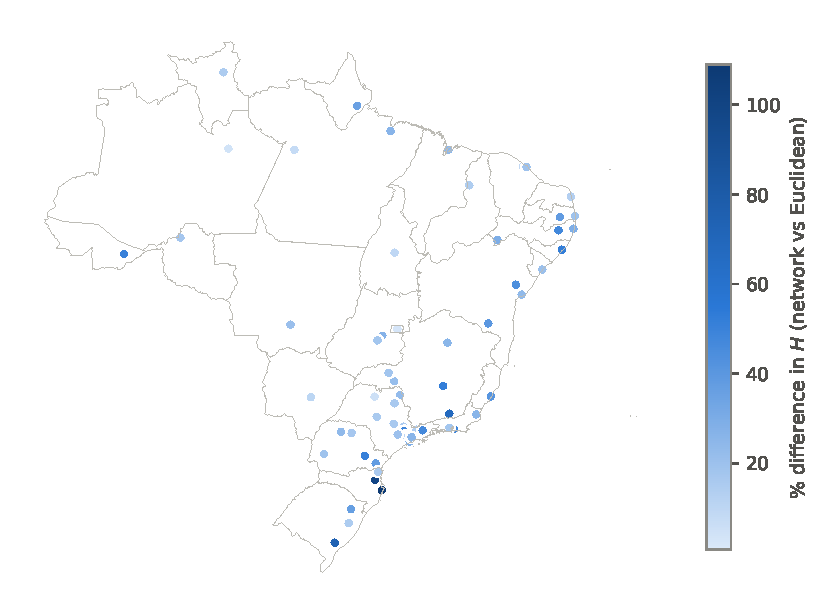
\includegraphics[width=0.72\textwidth]{figures/fig4_map_pdH.pdf}
\caption{Relative difference between network and Euclidean $H$ (\%) by municipality.}\label{fig:map}
\end{figure}

These results are robust to the kernel. With 1-km or 3-km bandwidths, an exponential kernel, or the
single-group dissimilarity and entropy indices for the \emph{preta}+\emph{parda} population, network-based
segregation remains higher in almost every city (Appendix Table~\ref{tab:robust}). The exception is the isolation
index, which changes little under either metric (its mean relative difference is below 2\% in every
specification).

\paragraph{Population-matched environments.} They are not robust, however, to holding the size of local
environments constant. Walking reaches far fewer people than a straight line: the mean 2-km network environment
contains \envPopRatio\% of the (kernel-weighted) population of the corresponding Euclidean environment (median
across cities), with a range of \ratioMin--\ratioMax\%. When each tract's Euclidean radius is shrunk until its
environment holds the same population as its network environment (median radius \medianPopmatchB~m), the gap
disappears. The mean relative difference becomes \meanPdHPopmatch\%, network $H$ exceeds the matched Euclidean $H$
in only \sharePositivePopmatch\% of cities, and the ranking under the two metrics becomes practically identical
(Spearman \spearmanPopmatch). The same holds for the single-group indices (Table~\ref{tab:robust}). In Brazilian
cities, therefore, the network--Euclidean gap is almost entirely a difference in the \emph{scale} of local
environments, as \citet{saporito2026reconsidering} argued for US cities, rather than evidence that the street
network separates groups beyond what a smaller neighbourhood would.

\subsection{Which network characteristics explain the gap?}

Figure~\ref{fig:clustermap} shows the correlation structure of the topology measures. As in
\citet{knaap2024segregated}, one cluster groups meshedness, gamma, streets per node and the share of 4-way
intersections (connectivity). A second groups circuity, dead-end share and self-loops (a dendritic, winding
fabric). A third groups size and density. Configurational fragmentation $F$ is nearly uncorrelated with all of
them. The relative gap belongs with the dendritic cluster: it rises with the dead-end share (Spearman
\rhoDeadEndPdH) and is essentially unrelated to $F$ (\rhoFragPdH).

\begin{figure}[htbp]
\centering
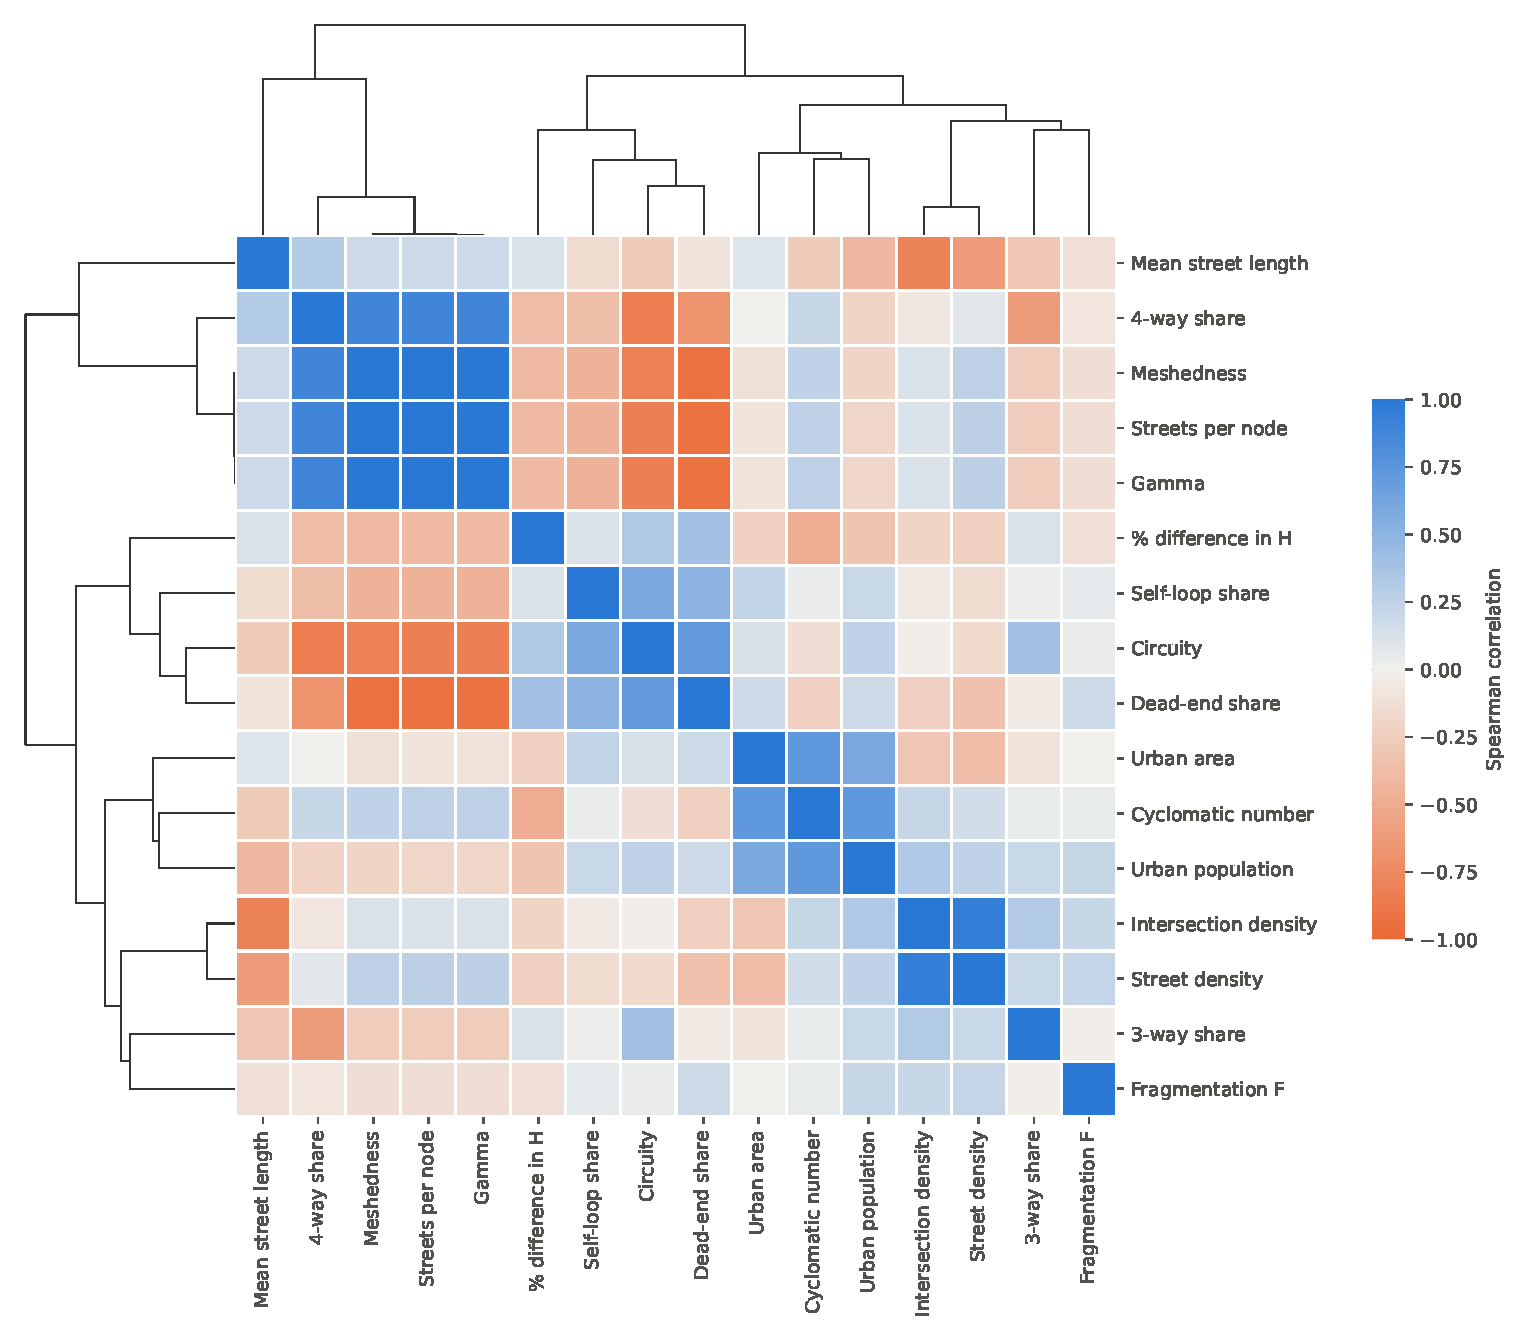
\includegraphics[width=0.8\textwidth]{figures/fig5_clustermap.pdf}
\caption{Spearman correlations among street-network topology measures, city size and the relative gap in
$H$, hierarchically clustered.}\label{fig:clustermap}
\end{figure}

Table~\ref{tab:models} reports the regressions. In all four models the dead-end share is positively associated
with both the absolute and the relative gap, and the level of Euclidean segregation is strongly associated with
the absolute gap (positively) and the relative gap (negatively). The negative association with the relative gap
means that low-segregation cities show larger relative differences, although the absolute differences there are
small. The cyclomatic number is negatively associated with the relative gap, consistent with more redundant
networks approximating unconstrained movement. Circuity, meshedness, intersection density and the
cyclomatic$\times$circuity interaction are not significant once the dead-end share is included. Meshedness and
the dead-end share are strongly collinear (variance inflation factors of 12.7 and 9.4), so their separate
coefficients should be read with caution. Adding fragmentation $F$ does not improve the fit: its coefficient is
small, negative and not significant, and the adjusted $R^2$ falls slightly. Figure~\ref{fig:frag} makes the
same point visually.

\begin{table}[htbp]
\centering\small
\caption{OLS models of the absolute ($\Delta H$) and relative (\%$\Delta H$) gap. K\&R: the specification of
\citet{knaap2024segregated}; +$F$: adding configurational fragmentation. Standardised (z) or logged regressors;
HC3 standard errors in parentheses. * $p<0.1$, ** $p<0.05$, *** $p<0.01$.}\label{tab:models}
\begin{tabular}{lrrrr}
\toprule
 & $\Delta H$ (K\&R) & $\Delta H$ (+$F$) & \%$\Delta H$ (K\&R) & \%$\Delta H$ (+$F$) \\
\midrule
Intersection density (log) & 0.0031 & 0.0030 & 14.34 & 13.66 \\
 & (0.0038) & (0.0039) & (9.46) & (9.39) \\
Circuity & 0.0001 & -0.0004 & 21.36 & 15.51 \\
 & (0.0072) & (0.0069) & (25.71) & (24.12) \\
Meshedness & 0.0015 & 0.0016 & -0.21 & -0.10 \\
 & (0.0018) & (0.0018) & (5.59) & (5.45) \\
Cyclomatic number (log) & -0.0017 & -0.0017 & -6.75** & -6.38* \\
 & (0.0011) & (0.0011) & (3.36) & (3.34) \\
Dead-end share & 0.0025** & 0.0026** & 9.14** & 9.68** \\
 & (0.0012) & (0.0012) & (4.46) & (4.30) \\
Population density (log) & -0.0027 & -0.0025 & -11.69* & -10.15 \\
 & (0.0022) & (0.0023) & (6.79) & (6.80) \\
$H$, Euclidean & 0.0030*** & 0.0030*** & -6.29*** & -6.40*** \\
 & (0.0005) & (0.0006) & (1.69) & (1.66) \\
Cyclomatic (log) $\times$ circuity & 0.0001 & 0.0002 & -2.23 & -1.58 \\
 & (0.0008) & (0.0007) & (2.87) & (2.68) \\
Fragmentation $F$ &  & -0.0002 &  & -2.16 \\
 &  & (0.0004) &  & (1.65) \\
Intercept & 0.0289** & 0.0277** & 121.95** & 109.01** \\
 & (0.0115) & (0.0127) & (47.90) & (50.25) \\
\midrule
$N$ & 91 & 91 & 91 & 91 \\
Adj. $R^2$ & 0.481 & 0.476 & 0.466 & 0.471 \\
\bottomrule
\end{tabular}

\end{table}

\begin{figure}[htbp]
\centering
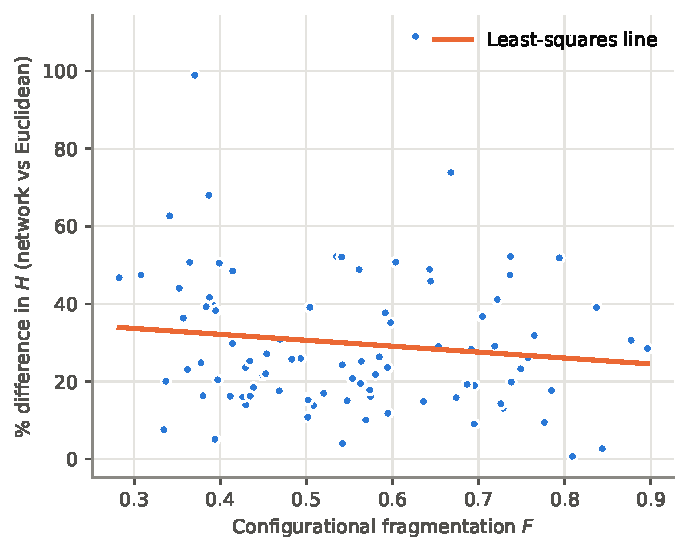
\includegraphics[width=0.55\textwidth]{figures/fig6_fragmentation.pdf}
\caption{Configurational fragmentation $F$ and the relative gap in $H$.}\label{fig:frag}
\end{figure}

The population-matched results suggest how topology matters. The share of the Euclidean population that is
reachable on foot is itself strongly associated with network form: it is lower where dead ends
(\rhoDeadEndRatio) and circuitous streets (\rhoCircuityRatio) are common and higher where the network is meshed
(\rhoMeshRatio), but it is unrelated to fragmentation (\rhoFragRatio). The gap is in turn larger where that
share is smaller (\rhoRatioPdH). Street topology thus shapes measured segregation mainly by setting the
effective scale of the neighbourhood.
